\chapter{Interacción \ac{CME}\index{Coronal Mass Ejection} - CME}
\begin{flushright}
\item \textit{''Contempla las estrellas y aprende de ellas
la verdadera forma de honrar al Maestro.
En su silencio eterno, siguen su curso
según las leyes de Newton.''}

-Albert Einstein
\end{flushright}
%Mencionar los diferentes casos en los que las \acp{CME}\index{Coronal Mass Ejection} pueden interactuar, bajo diferentes parámetros, como la velocidad, dirección, tamaño.

La interacción entre \acp{CME}\index{Coronal Mass Ejection} ha sido observada desde los años 2000 con ayuda del Large Angle and Spectrometric Coronagraph Experiment – LASCO –, además de tener mediciones in situ desde 1970s.



La interacción entre dos o más \acp{CME}\index{Coronal Mass Ejection} está asociada a:

\begin{itemize}
    \item Reconexión magnética
\item Intercambio de momentum
\item Choque magnetosónico
\item SEPs (interacción shock-shock)
\item Ondas de radio inusuales (electrones acelerados)
\end{itemize}

\section{Variación de las propiedades en la interacción}
En la interacción entre CMEs, éstas pueden cambiar sus propiedades tales como su velocidad, su tamaño, su taza de expansión, su dirección de propagación, su tiempo de llegada a la Tierra y su probabilidad de impacto con ésta ultima, así como el campo magnético interno en cada CME.

Se considera términos como el coeficiente de restitución y la colisión inelástica vs. elástica vs. superelástica. Donde el coeficiente de restitución se entiende como el parámetro que clasifica la cantidad de rebote en una colisión y se define como:
\begin{equation}
   e=\frac{{v_{\text{después,2}}-v_{\text{después,1}}}}{v_{\text{antes,1}}-v_{\text{antes,2}}} 
\end{equation}
En donde $v_{\text{después,2}}$ y $v_{\text{después,1}}$ son las velocidades de los cuerpos 2 y 1 después de la colisión, mientras que $v_{\text{antes,1}}$ y $v_{\text{antes,2}}$ son las velocidades de los cuerpos 1 y 2 antes de la colisión. Véase que el numerador es la velocidad relativa después de la colisión y el denominador es la velocidad relativa antes de la colisión. Ahora bien, este coeficiente de restitución permite clasificar las interacciones CME-CME según su tipo de colisión, así:
\begin{itemize}
    \item Con $e=1$ es una colisión elástica que es un colisión ideal, es decir, sin pérdidas de energía.
\item Con $e<1$ es una colisión inelástica en donde hay pérdida de energía. 
\item Con $e>1$ es una colisión superelástica lo que indica una ganancia de energía.
\end{itemize}



A lo largo de la propagación de las \acp{CME}\index{Coronal Mass Ejection} en interacción a lo largo del viento solar interplanetario Sol-Tierra, pueden tomar diferentes formas:

\begin{itemize}
    \item Interacción únicamente de los dos choques de onda de las CMEs, pero sin interacción de la eyección.
\item Una onda de choque de una \ac{CME}\index{Coronal Mass Ejection} secundaria interactúa con la eyección de masa de una \ac{CME}\index{Coronal Mass Ejection} anterior. En este caso la presencia de una onda de choque afecta la velocidad final de la \ac{CME}\index{Coronal Mass Ejection} resultante de la interacción entre CMEs, así pues si no hay presencia de una onda de choque la velocidad final será determinada por la \ac{CME}\index{Coronal Mass Ejection} más lenta, mientras que cuando si se encuentra una onda de choque la velocidad será definida principalmente por la \ac{CME}\index{Coronal Mass Ejection} más rápida. 


Además, la onda de choque precedente a la primera \ac{CME}\index{Coronal Mass Ejection} se verá afectada al interactuar con las partes de esta primera CME, por lo que un choque se propaga más rápido dentro de una nube magnética, ya que allí la velocidad magnetosónica es elevada en su interior debido a la densidad del viento solar en esa región.
Se puede dividir la interacción de la onda de choque secundaria con la \ac{CME}\index{Coronal Mass Ejection} primordial en 4 fases, según lo toma \cite{lugaz-2017}:
\begin{itemize}
    \item Cuando el choque se propaga a través de una región con una baja densidad de viento solar, por lo que se le permite ir más rápido.
\item Cuando el choque entra en una nube magnética, disminuyendo su relación de compresión y aumentando su velocidad vista desde un marco en reposo; sin embargo, si el choque no es lo suficientemente rápido podría disiparse dentro de la nube magnética.
\item Cuando el choque llega a la capa densa de la \ac{CME}\index{Coronal Mass Ejection} y se desacelera.
\item Cuando ocurre la fusión de los dos choques, que según la magnetohidrodinámica, terminarán superponiéndose e intensificándose. 

\end{itemize}

\item Las eyecciones magnéticas sucesivas pueden interactuar y/o reconectarse, después de que el choque de la segunda \ac{CME}\index{Coronal Mass Ejection} liberada haya alcanzado a la primera, como lo toma \cite{lugaz-2005}, la interacción del segundo choque con la primera \ac{CME}\index{Coronal Mass Ejection} se presenta en 4 fases.
\begin{itemize}
    \item La primera fase es la preparación del escenario, cuando las dos \acp{CME}\index{Coronal Mass Ejection} son liberadas con un intervalo de tiempo de 10 horas entre cada una de las CMEs, en donde la primera \ac{CME}\index{Coronal Mass Ejection} genera perturbaciones en el viento solar para que luego la segunda \ac{CME}\index{Coronal Mass Ejection} o el choque de retaguardia pase por allí, encontrando un viento solar perturbado con menor densidad y mayor campo magnético. Justo cuando se libera la segunda CME, el choque de la primera \ac{CME}\index{Coronal Mass Ejection} está a 43.9 radios solares con una velocidad al rededor de los 625 $Km/h$ y su nube magnética correspondiente está a 32.3 radios solares con una velocidad de 500 $Km/s$. 

    Además, la primera \ac{CME}\index{Coronal Mass Ejection} liberada presenta un incremento de masa debido al arrastre de masa coronal ambiental, eliminando parte de la masa de plasma de fondo. Por lo que su velocidad se verá afectada justo cuando empieza su ascenso junto con el viento solar, por lo que su velocidad viene dada a través de las relaciones de Rankine-Hugoniot, teniendo que:
\begin{equation}
    V_{shock}=\frac{\rho_{1}U_{1}-\rho _{0} U_{0}}{\rho_{1}-\rho_{0}}
    \label{Vshock}
\end{equation}
Donde $U_1$ es la velocidad del plasma medida aguas abajo del choque en el marco de referencia del mismo, al igual que $U_0$ es la velocidad del plasma aguas arriba medida desde el choque. Con el índice 0 refiriéndose a la parte aguas arriba (upstream) o en las regiones en donde aún no pasa el choque y el índice 1 a las partes aguas abajo (downstream) o en donde ya pasó el choque. Lo que producirá finalmente, que el choque del segundo \ac{CME}\index{Coronal Mass Ejection} vaya más rápido (entre 150 y 200 km/s) a pesar de que tanto la primera como la segunda \ac{CME}\index{Coronal Mass Ejection} tienen la misma velocidad inicial, esto debido a que el primer choque se vio afectado por el arrastre de viento solar, aumentando el gradiente de presión hacia afuera y la velocidad de modo rápido para el segundo CME, llegando a que la segunda \ac{CME}\index{Coronal Mass Ejection} sobrepase a la primera lentamente.

\item La segunda fase ocurre luego de 14 horas en donde el choque del segundo \ac{CME}\index{Coronal Mass Ejection} con una velocidad de 1150 $km/s$ y un factor de compresión al rededor de 3 (con $r=\frac{\rho_{1}}{\rho_{0}}=3$ significa que la densidad del plasma aguas abajo es 3 veces más grande que la densidad aguas arriba) alcanza a la nube magnética del primer CME, lo que genera una interacción nube magnética-choque durante 8 horas aproximadamente, el plasma de la nube magnética experimenta una transición de un plasma dominado por la presión (plasma a altas temperaturas) a uno dominado por el magnetismo (con una intensidad del campo magnético alta), esto según el parámetro \hyperref[beta]{$\beta$}. 

Donde la \hyperref[Valfvenica]{velocidad Alfvénica} es la velocidad a la que se propagan las perturbaciones magnéticas en el plasma, mientras que la velocidad sónica es la velocidad a la que se propagan las perturbaciones de presión en el plasma, dada por:
\begin{equation}
    V_{sónica}=\sqrt{ \frac{\gamma p}{\rho} }
\end{equation}

Donde $\gamma$ es la constante adiabática del gas, $p$ es la presión del plasma y $\rho$ es su densidad. Por lo que en \cite{lugaz-2005} se dice que cuando el segundo choque interactúa con la nube magnética del primer CME, se presenta un aumento de $\beta$ lo que se traduce en una disminución de la temperatura tal que genera una presión térmica 100 veces menor a la presión magnética directamente en aguas arriba del choque, por lo que el campo magnético dominará en esa región. Por otro lado, también indica que la densidad aguas arribas es menor, por lo que el segundo choque se propagará en un medio 15 veces más tenue lo que permitirá una aceleración del mismo hasta los 1572 $km/s$ , además la velocidad Alfvénica se incrementa 8 veces, lo que significa que el campo magnético en conjunto con la densidad del plasma se reconfiguran de tal forma que ocurriera ese incremento, llegando a un campo magnético más intenso lo que lleva a la reducción de la relación de compresión del choque. La velocidad sónica se mantiene similar, lo que indica que las variaciones en la presión del plasma y en su densidad son directamente proporcionales, de tal forma que su razón se mantenga casi igual. 
Por otro lado, está el parámetro Mach de Alfvén, el cual permite ver si las perturbaciones magnéticas se mueven más o menos rápido que el mismo plasma, definido como:
\begin{equation}
M_{A}=\frac{V}{V_{a}}
\end{equation}
Donde $V$ es la velocidad característica del viento solar y \hyperref[Valfvenica]{$V_A$} es la velocidad de Alfvén. En este caso el plasma aguas arriba es sub-Alfvénico localmente, es decir que tiene un número Mach menor a 1: $M_A<1$, al rededor de 0.81, según \cite{lugaz-2005}.
Una vez que el choque interactúe con la nube magnética, presentará una desaceleración debido al aumento de la densidad del plasma aguas arriba, afectando la velocidad del choque \hyperref[Vshock]{$V_{shock}$}, ya que $\rho_0$ será mayor por lo que la velocidad disminuirá.

\item La tercera etapa ocurre cuando el choque de la segunda \ac{CME}\index{Coronal Mass Ejection} avanza hasta encontrarse con la vaina que es la estructura densa que recubre la nube magnética de la primera CME. Recordando que la nube magnética y la sheath están separas por una discontinuidad, en donde se puede considerar sin magnetización, de tal forma que la presión del plasma es la que domina completamente, es decir que el parámetro \hyperref[beta]{$\beta$} es mayor o igual a 2000, indicando que la presión térmica es 2000 veces más intensa que la presión magnética.
Además, la velocidad del sonido en esta región es más grande que en la nube magnética, al rededor de $1.5$ veces más rápida y la densidad del plasma 2 veces más grande que la densidad de la nube magnética. Ahora bien, como la velocidad del choque cambia debido a las densidades aguas arriba y aguas abajo, se presentará una desaceleración del choque, puesto que entra a una región con una densidad mayor lo cual según la ecuación de \hyperref[Vshock]{$V_{shock}$}, indica que la velocidad disminuirá de 850 a 700$km/s$, aun así la velocidad del choque es suficiente como para rebasar al choque de la primera CME, todo esto mencionado en \cite{lugaz-2005}.

\item Para la última fase se tiene que los dos choques interactúan formando un nuevo choque que se propaga hacia el viento solar no perturbado, para luego llegar hasta la Tierra, seguido de la primera y segunda nube magnética. p.4
El choque resultante es más fuerte que los otros dos anteriores, ya que tiene una relación de compresión de 3.59 comparado con el 1.52 y 3.13 del segundo y del primer choque. Así pues, este nuevo choque generado calienta las regiones por donde va pasando al mismo tiempo que disminuye la densidad del plasma en las regiones aguas abajo del nuevo choque.
\end{itemize}

También se presenta la interacción entre las dos nubes magnéticas recordando que la primera ya interactuó con el choque de la segunda, por lo que la primera nube se comprimió y se aceleró antes de entrar en contacto con la segunda. Por otro lado, en \cite{lugaz-2005} se muestra una reconexión y un choque inverso asociado con la colisión de las dos nubes magnéticas. Cuando las dos nubes magnéticas colisionan ya ha pasado el segundo choque a través de la primera lo que significa que este modificó la velocidad de la nube magnética aguas abajo, lo que lleva a que se presente una zona de reconexión suave entre las dos nubes magnéticas. Esta zona de reconexión tiene un ancho entre 2 y 3 radios solares, con una velocidad en su frente similar a la velocidad aguas abajo del choque que acaba de pasar por la primera \ac{CME}\index{Coronal Mass Ejection} (esta velocidad empezará a disminuir a medida que el choque se aleje de ella), y una velocidad posterior similar a la velocidad en el frente de la segunda CME, lo que significa que la zona de reconexión presenta una compresión, ya que su parte trasera se mueve más rápido que su parte frontal. Además, la reconexión disminuye la velocidad Alfvénica en esa zona lo que llevaría a que la diferencia de velocidades frontales y posteriores de la zona de reconexión se volviera Super-Alfvénica localmente, lo que a su vez generaría un choque inverso de modo rápido. Este choque reduce la velocidad posterior de la zona de reconexión así como el frente de la segunda nube magnética, además de aumentar la temperatura, la densidad y el campo magnético. En la propagación del choque inverso a lo largo de la segunda nube magnética, se desacelera perdiendo fuerza y efectividad hasta desaparecer en la parte posterior de la segunda nube magnética. 

Ahora, la segunda nube magnética presenta una evolución en el tiempo, ya que debido a la colisión con la primera nube magnética presenta una desaceleración además de volver a desacelerarse posteriormente con la interacción con el choque inverso, mientras que la primera nube presenta una aceleración resultante de la interacción con el segundo choque p.9, cabe señalar que antes de esta interacción la primera nube se estaba desacelerando debido a su expansión

\item Ni las \acp{CME}\index{Coronal Mass Ejection} ni sus choques llegan a interactuar. Estos casos afectan el flujo de SEPs y la propagación de la segunda CME, la cual sale de la misma región pero con una diferencia de tiempo considerable. Por lo que, el primer \ac{CME}\index{Coronal Mass Ejection} eliminó parte del viento solar que había en la trayectoria de la segunda \ac{CME}\index{Coronal Mass Ejection} lo que indicaría que la segunda \ac{CME}\index{Coronal Mass Ejection} no presentaría tanta desaceleración como la primera. Así pues, se evidenciaría que el tiempo de tránsito se reduce por una presencia de dos \acp{CME}\index{Coronal Mass Ejection} sin interacción, la primer \ac{CME}\index{Coronal Mass Ejection} desplaza el material frente a ella despejando el camino para que el segundo alcance una mayor velocidad al desplazarse por las regiones previamente despejadas.
\end{itemize}

\section{Estructuras resultantes de la interacción}
La estructura más simple resultante es una múltiple nube magnética, que consiste en una nube magnética precedida por otras. Una nube magnética está asociada con las CMEs, una nube magnética es una estructura coherente (que mantiene su estructura y forma en el tiempo), grande y compacta de campo magnético que viaja a través del medio interplanetario.
Las características de una nube magnética consisten en:
\begin{itemize}
    \item Tener un campo magnético intenso, mayor al del medio interplanetario
\item Baja temperatura del plasma en comparación con el viento solar normal
\item Baja beta del plasma, es decir que:
\begin{equation}
\beta= \frac{P_{\text{térmica}}}{P_{\text{magnética}}}\ll 1 \label{beta}
\end{equation}
Lo que significa que el campo magnético domina sobre la presión térmica, ya que la presión magnética es mayor (la nube magnética es una estructura coherente) y la presión térmica es menor (el plasma es más frío). Donde $P_{\text{Térmica}}=nkT$, con $n$ la densidad molar del plasma, $k$ es la constante de Boltzmann y $T$ es la temperatura del plasma. Por otro lado, la $P_{\text{Magnética}}=\frac{B²}{2 \mu_{0}}$ con $B$ la intensidad del campo magnético y $\mu_{0}$ es la permeabilidad del vacío.
Recordando que el parámetro adimensional $\beta$ permite comparar la presión térmica del plasma con la presión magnética del campo magnético contenido en el mismo,, permitiendo identificar su estabilidad, así:
\begin{itemize}
    \item $\beta\ll 1$: El campo magnético domina sobre la presión térmica
\item $\beta=1$: Ambas presiones son comparables
\item $\beta>>1$: La presión térmica domina, por lo que el campo magnético tiene poca influencia
\end{itemize}
\end{itemize}


Otra estructura que se puede formar son las eyecciones complejas, en donde las nubes magnéticas no son distinguibles entre sí, lo que indica que tendrá un campo magnético complejo, a diferencia de una múltiple nube magnética. Otra estructura sería los eventos de larga duración, en donde las nubes magnéticas están muy separadas entre sí, lo que evita que se fusionen.

\section{Interacción CME-CME y los eventos de SEPs}

%hablar sobre qué son las SEPs

Las partículas solares energéticas (Solar Energetic Particles SEPs) están relacionadas con dos fenómenos principales:
\begin{itemize}
    \item Las Llamaradas solares
\item Las \acp{CME}\index{Coronal Mass Ejection} y sus ondas de choque
\end{itemize}

La forma de medir la intensidad de SEPs que presenta una erupción es a través de las unidades de flujo de partículas, definido como:
\begin{equation}
    1 \text{pfu}=1~\text{protón por} ~ cm^{-2}s^{-1}\text{sr}^{-1}
\end{equation}

%explicar que es sr

Ahora, se cree que la aceleración de las SEPs ocurre dentro de los primeros 10 Radios solares, lo que hace que la interacción entre los choques de las \acp{CME}\index{Coronal Mass Ejection} sea menos probable de causar esta aceleración, puesto que la mayoría de las interacciones ocurren fuera de esos 10 radios solares.

La interacción entre dos ondas de choque dentro de un medio rico en partículas semilla y en turbulencias puede aumentar la energía máxima de las partículas. Además, el 60$\%$ de las \acp{CME}\index{Coronal Mass Ejection} gemelas conducen a grandes eventos de SEPs, mientras que solo el 20$\%$ de \acp{CME}\index{Coronal Mass Ejection} simples conducen a grandes eventos de SEPs, según \cite{lugaz-2017}. Por otro lado, la geometría del frente del \ac{CME}\index{Coronal Mass Ejection} también puede afectar la producción de SEPs y la energía con la que se liberan.

%hablar de partículas semilla y de turbulencias

Los electrones del plasma presentan una aceleración en la interacción CME-CME que es posible detectar a través de las señales de ondas electromagnéticas en el rango de las ondas de radio, esto es porque un electrón emite radiación cuando es acelerado. Así pues, cuando se miden o se detectan señales de radio se asocian con procesos de aceleración de partículas. Se ha encontrado que la emisión de señales de radio de tipo II coinciden con la interacción entre el frente de una \ac{CME}\index{Coronal Mass Ejection} secundaria y una primera \ac{CME}\index{Coronal Mass Ejection} ocurrida antes. 

Cabe señalar los diferentes tipos de emisiones de ondas de radio debido a electrones acelerados, tenemos:
\begin{itemize}
    \item Tipo I: Provenientes de emisiones casi continuas, con ráfagas breves y estrechas en frecuencia que se asocian a regiones activas solares con pequeños eventos de reconexión. Su duración va desde horas hasta días.
    \item Tipo II: Emisiones lentas producidas por ondas de choque en la corona solar o en el medio interplanetario, típicamente impulsadas por una \ac{CME}\index{Coronal Mass Ejection} rápida. Se interpretan como electrones acelerados en el frente de choque que excitan ondas de Langmuir relacionadas con la conversión a ondas de radio. %hablar sobre las ondas de Langmuir
    Es una señal de que hay un frente de choque presente, útil para diagnosticar la velocidad de propagación de las CMEs.
    \item Tipo III: Provenientes de ráfagas muy rápidas de alta frecuencia a baja frecuencia generadas por haces de electrones acelerados que viajan por líneas de campo magnético abiertas o cuasi-abiertas hacia el espacio interplanetario.Además, asociadas a reconexiones magnéticas rápidas, como en Llamaradas solares durando segundos.
    \item Tipo IV: Relacionada con la emisión de banda ancha más lenta y sostenida asociada a plasma atrapado en estructuras magnéticas grandes como lóbulos cerrados de \acp{CME}\index{Coronal Mass Ejection} durando minutos u horas.
    \item Tipo V: Es una emisión de fondo difusa, más suave y continua, que sigue a una ráfaga tipo III que dura al rededor de decenas de segundos, se cree que es generado por electrones remanentes más térmicos.
\end{itemize}

En \cite{gonzalez-esparza-2004} se habla sobre un modelo magnetohidrodinámico en 1D y 2D que busca estudiar la interacción entre CMEs, lejos de la superficie solar para evitar las reconexiones magnéticas. Así pues, para hacer la simulación se emiten dos CMEs, la primera más lenta que la segunda de tal forma que en un momento la segunda pase a la primera y genere la interacción. Utilizan el código ZEUS-3-D, el cual resuelve las ecuaciones magnetohidrodinámicas ideales, es decir, que no son resistivas ni viscosas, pero tomando que la contribución magnética es mínima.

Ahora, generan las características del viento solar especificando su velocidad, densidad y temperatura en la frontera en donde se puede despreciar los efectos magnéticos, es decir, a 18 radios solares según el artículo, para luego dejar que evolucionara y llegara a un estado estacionario. En seguida, se lanzan las perturbaciones de tipo eyección las cuales presentan una velocidad y generan pequeños incrementos en densidad y temperatura.

Así pues, la simulación se puede generar en 1D o en 2D. Para 1D se inyectaron 2 \acp{CME}\index{Coronal Mass Ejection} con intervalo de 15 horas, generando datos a intervalos de 20, 40 y 70 horas después del primer lanzamiento (los resultados de la simulación se muestran en la figura \ref{fig:1D}), la primera \ac{CME}\index{Coronal Mass Ejection} con una velocidad de 450 $km/s$ y la segunda a 800 $km/s$, en un viento solar con una velocidad de 400 $km/s$, además se tiene en cuenta las características del viento solar a una distancia de 0.083 AU, en donde se colocan condiciones de frontera (tanto para 1D como para 2D) así como a 1AU, mostradas en la tabla \ref{fig:condiciones de contorno}.


%convertir las imagenes de tablas a tablas
\begin{figure}[H]
    \centering
    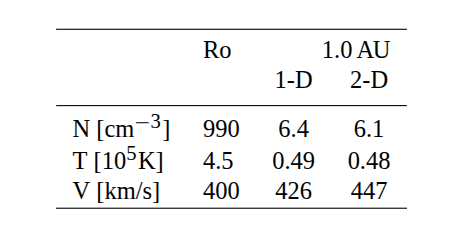
\includegraphics[width=0.4\linewidth]{imag/condiciones de contorno.png}
    \caption{Características del ambiente del viento solar a 0.083AU y a 1AU}
    \label{fig:condiciones de contorno}
\end{figure}

Por otro lado, las condiciones de las \acp{CME}\index{Coronal Mass Ejection} generadas en la simulación de 1D, se muestran en la tabla \ref{fig:caracteristicas de las CMEs}.
\begin{figure}[H]
    \centering
    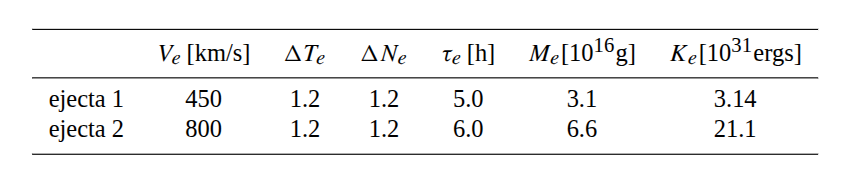
\includegraphics[width=0.7\linewidth]{imag/condicones CMEs.png}
    \caption{Características de las CMEs, con $V_e$ las velocidades de las CMEs, incremento de la densidad $\Delta N_e=N_e/N_0$ y de la temperatura $\Delta T_e=T_e/T_0$, $\tau_e$ como la duración de la generación de la CME, $M_e$ es la masa total y $U_e$ es la energía cinética total.}
    \label{fig:caracteristicas de las CMEs}
\end{figure}

\begin{figure}[H]
    \centering
    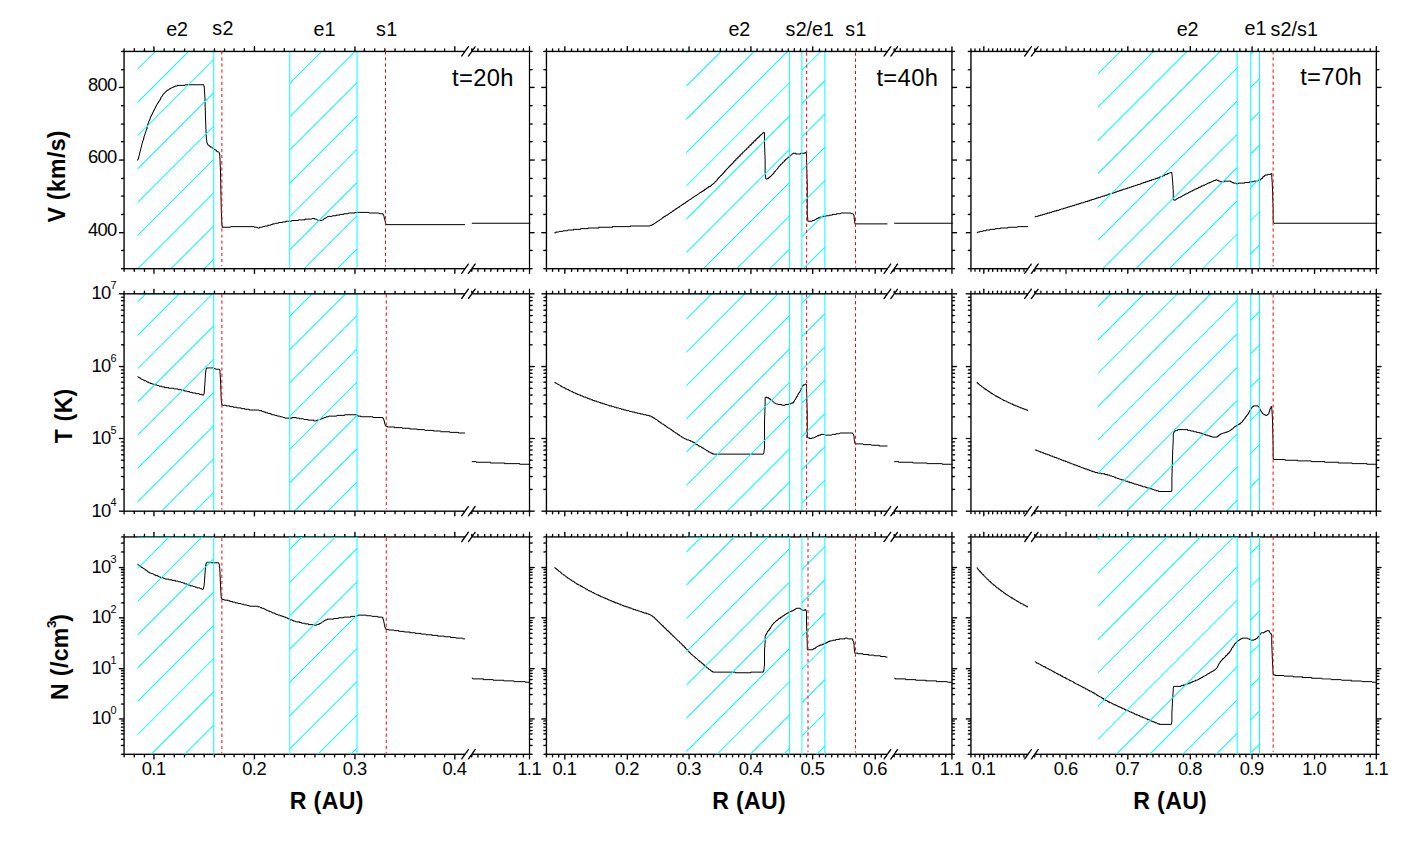
\includegraphics[width=0.8\linewidth]{imag/1D.png}
    \caption[Resultados de la simulación de una CME a 1D hecha por \cite{gonzalez-esparza-2004}]{Resultados de la simulación a 1D, con intervalos de tiempo diferentes, donde e1 y e2 son la primera y segunda CME, respectivamente; s1 y s2 son las ondas de choque de las \acp{CME}\index{Coronal Mass Ejection} 1 y 2, respectivamente.}
    \label{fig:1D}
\end{figure}

Ya para 2D se tiene que las condiciones de las \acp{CME}\index{Coronal Mass Ejection} generadas son las mostradas en la tabla \ref{fig:condiciones 2D}.
\begin{figure}[H]
    \centering
    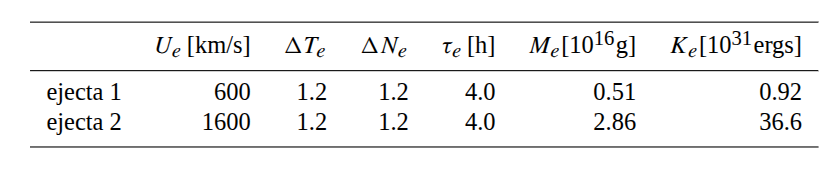
\includegraphics[width=0.7\linewidth]{imag/2D condiciones.png}
    \caption{Condiciones de las \acp{CME}\index{Coronal Mass Ejection} utilizadas en la simulación en 2D}
    \label{fig:condiciones 2D}
\end{figure}
Para esta simulación se tiene en cuenta la dirección de propagación de las CMEs, así como su tamaño angular. También, el intervalo de tiempo entre los lanzamientos de las 2 \acp{CME}\index{Coronal Mass Ejection} es de 15 horas. Los resultados de esta simulación se muestran en las figuras \ref{fig:simulación 2D1} y \ref{fig:simulación 2D2}.

\begin{figure}[H]
    \centering
    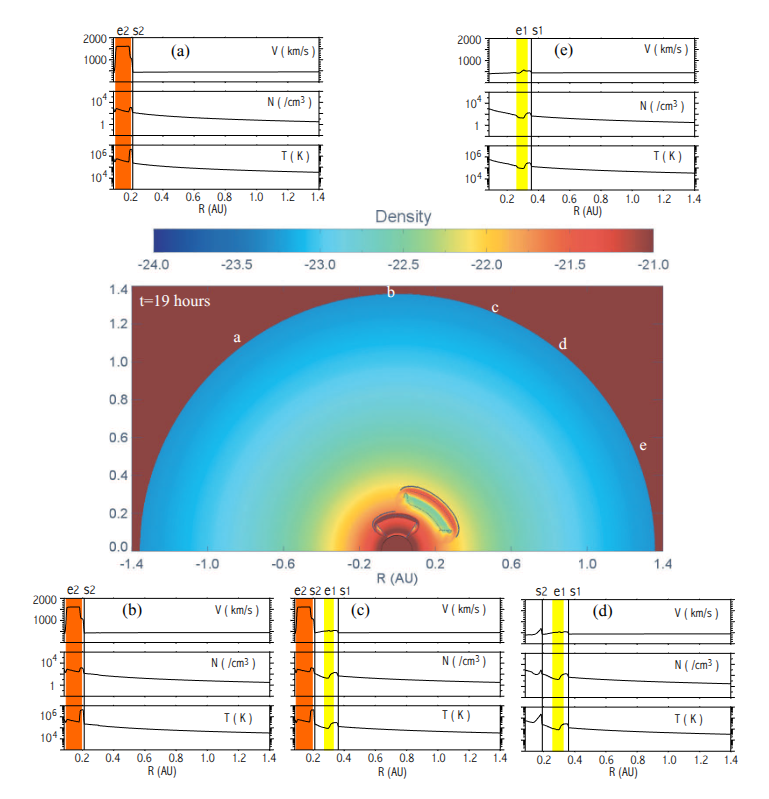
\includegraphics[width=0.8\linewidth]{imag/2D1.png}
    \caption[Simulación en 2D de dos CMEs hecha por \cite{gonzalez-esparza-2004}]{Simulación en 2D, las gráficas muestran el comportamiento de la velocidad, la densidad y la temperatura del viento solar en diferentes direcciones, 19 horas después del lanzamiento de la CME1}
    \label{fig:simulación 2D1}
\end{figure}

\begin{figure}[H]
    \centering
    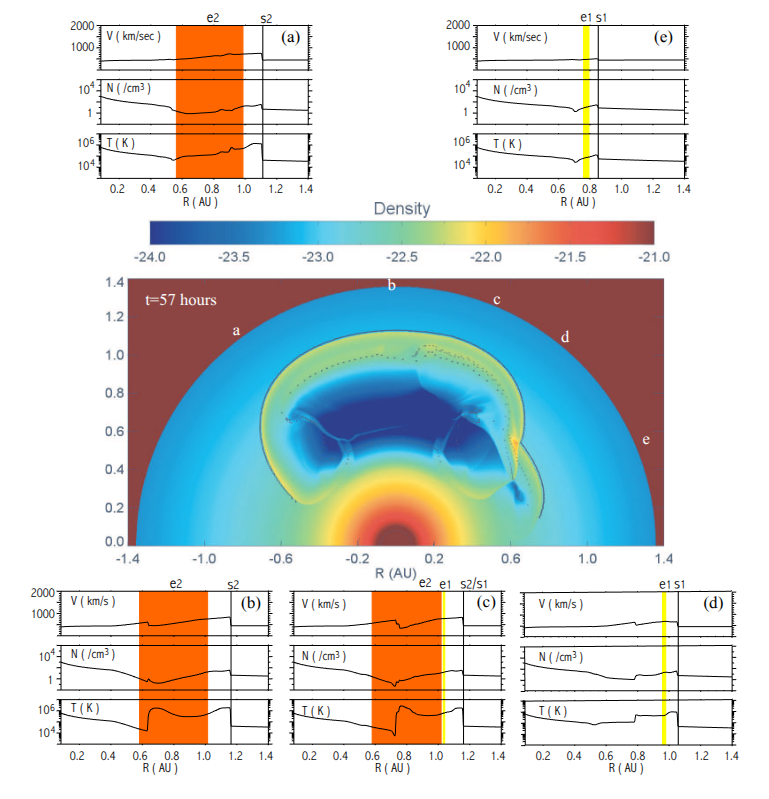
\includegraphics[width=0.8\linewidth]{imag/2D2.png}
    \caption[Simulación en 2D de dos CMEs hecha por \cite{gonzalez-esparza-2004}, 29 horas después del lanzamiento de la primera CME]{Similar a la figura \ref{fig:simulación 2D1} pero 29 horas después del lanzamiento de la CME1}
    \label{fig:simulación 2D2}
\end{figure}
Se evidencia que la complejidad de la simulación aumenta cuando se utilizan 2 dimensiones. Cabe señalar que se utiliza un modelo hidrodinámico, ya que la interacción ocurre en regiones en donde no hay re-conexión magnética. Además, el paper llega a la conclusión de que hay una transferencia de momentum entre las CMEs, en donde la CME2 con una velocidad mayor transfiere momentum a la CME1 a través de la onda de choque de la CME2 que comprime y acelera la CME1. Cuando llegan a 1AU, las dos \acp{CME}\index{Coronal Mass Ejection} llevan velocidades similares, pero la CME1 un poco más rápida que la CME2, además las ondas de choque se superponen y forman una única onda de choque más intensa.


Por otro lado, \cite{} realiza una simulación en 2.5D, es decir que considera dos dimensiones espaciales y la tercera dimensión la considera parcialmente, lo que reduce el gasto computacional de la simulación, la cual se basa en un modelo magnetohidrodinámico. La simulación busca ver el comportamiento de las nubes magnéticas, su interacción con otras nubes magnéticas y la formación de nubes múltiples en la heliosfera.
Para correr la simulación primero se modela una nube magnética como una linea de flujo en 2.5D. Cabe señalar que la simulación se realiza en coordenadas esféricas. Una vez modeladas las dos lineas de flujo, se les permite propagarse la primera con una velocidad menor a la segunda y separadas un intervalo de 12 horas entre la primera y la segunda.
El artículo reporta que la segunda \ac{CME}\index{Coronal Mass Ejection} tarde 18 horas en alcanzar a la primera CME, por lo que en ese momento interactúan y generan una nube magnética múltiple que llega hasta 1AU. Además, menciona que la segunda nube magnética se ve desacelerada debido a la interacción con la primera nube magnética, por lo que el tiempo de viaje de la nube magnética múltiple depende de la velocidad de la primera \ac{CME}\index{Coronal Mass Ejection} (lenta). 

